
\chapter{Formulations in linear elasticity}
\section{Strong formulation}	
	The equilibrium equations omitting concentrated body moments and the material law in linear elasticity for isotropic and homogeneous materials are:
	
	\begin{equation}
	b_i + \tau _{ij,j} = 0, \qquad \epsilon _{ij} = \frac{1}{E }[(1+\nu) \tau _{ij} - \nu \delta _{ij} \tau _{kk}].
	\end{equation}
	
	Since there is a linear relation between stresses and strains, strain tensor $\epsilon _{ij}$ derives itself from the displacement field, we can rewrite the equilibrium equations in function of the displacements. This leads to the \textbf{displacement-based finite element method}, the unknowns are the displacements. All the set of equations are encompassed under the \textbf{strong formulation} therminology, because they require to be satisfied \textbf{locally}, at each point of the domain V.
	
\subsection{Boundary conditions}
	The main classes of boundary conditions are: 
	
	\begin{itemize}
	\item[•] \textbf{essential boundary conditions} (Dirichlet): the displacement is prescribed on a portion of the external surface $S$, called $S_u$; \\
	
	\item[•] \textbf{natural boundary conditions} (Neumann): the contact force is imposed on another portion of the external surface $S$, called $S_t$. 
	\end{itemize}
	
\subsection{Mathematical properties of the governing equations}
	First, the \textbf{superposition principle} is respected by stresses, strains and displacements because linearity of the static and kinematic equations in linear elasticity (assuming small displacements/strains). Indeed if $\tau _{ij}^A$ and $\tau _{ij}^B$ are stress tensors associated to load cases A and B, $\tau _{ij}^A + \tau _{ij}^B$ is the solution for the load case A + B. \\
	
	Secondly, for given surface and body forces, the uniqueness of the solution for the governing equations is guaranteed. 
	
	\begin{proof}
	As a counterargument, let's assume that there exist two solution $u_i^{(1)}$ and $u_i^{(2)}$ and their difference $u_i ' = u_i^{(1)}-u_i^{(2)}$. Let's do the same for strains and stresses:
	
	\begin{equation}
	\epsilon _{ij} ' = \epsilon_{ij}^{(1)}-\epsilon _{ij}^{(2)}, \qquad \tau _{ij} ' = \tau _{ij}^{(1)}-\tau _{ij}^{(2)}.
	\end{equation}
	
	Since the body forces are external and identical for the two solutions, we get from the equilibrium equations:
	
	\begin{equation}
	\tau_{ij,j}^{(1)}-\tau_{ij,j}^{(2)} = \tau_{ij,j} ' = 0. 
	\end{equation}
	
	On the other hand, the strain energy of the difference is:
	
	\begin{equation}
	W' = \frac{1}{2}\int _V \epsilon _{ij} ' \tau _{ij} ' \, dV =  \frac{1}{2}\int _V \frac{1}{2} (u _{i,j} '+ u _{j,i} ') \tau _{ij} ' \, dV = \frac{1}{2}\int _V u' _{i,j} \tau _{ij} ' \, dV,
	\end{equation}
	
	by symmetry and as i, j are repeated. If we use integration by part and Gauss theorem, we get:
	
	\begin{equation}
	\begin{aligned}
	W' &= \frac{1}{2} \int _V (u' _{i} \tau ' _{ij})_{,j} \, dV - \frac{1}{2} \cancel{\int _V u' _{i} \tau ' _{ij,j} \, dV} \\
	&= \frac{1}{2} \oint _S u' _{i} \tau ' _{ij} n_j \, dV = \frac{1}{2} \oint _S u' _{i} \bar{\tau '} _{i}^{(n)} \, dV
	\end{aligned}
	\end{equation}
	
	To guarantee the uniqueness of the solution, so to have $W' = 0$, the boundary conditions must satisfy:
	
	\begin{enumerate}
	\item the displacement field $u_i$ is prescribed on the entire surface, leading directly to $u_i ' = 0$
	
	\item the contact forces $t_i ^{(n)}$ are imposed over the entire surface while overall equilibrium is satisfied, making $t_i ^{'(n)} = 0$
	
	\item displacements $u_i$ are prescribed on one part of the surface ($u_i = \bar{u}_i$ on $S_u$), while contact forces $\tau _i^{(n)}$ are imposed on the rest of the surface ($\tau _i^{(n)} = \bar{\tau} _i^{(n)}$ on $S_t$), so that either $u_i '= 0$ or $\tau _i^{(n)}= 0$. The $\bar{ }$ symbol indicates that the values are prescribed. 
	\end{enumerate}
	\end{proof}
	
	This explains why it is not allowed to impose both the displacement and the force on the same point and the same direction. Example on \autoref{fig:4.1}. 
	
	\begin{center}
	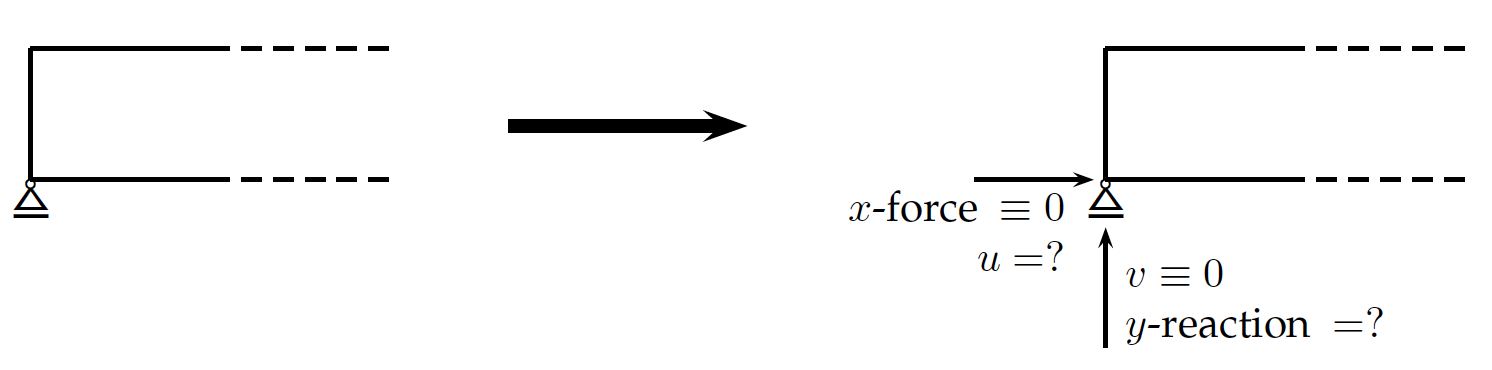
\includegraphics[scale=0.3]{ch4/1}
	\captionof{figure}{}
	\label{fig:4.1}
	\end{center}
	
\subsection{Linear elasticity governed by elliptic PDE's}
	A wide range of systems are governed by partially differential equatinos. It can be proven that the governing equations for linear elasticity constitute a set of \textbf{elliptic second-order partial differential equations}. An implication of this kind of system is that a small disturbance at one point P in the domain V has an impact on the whole body, and inversely a point P is influenced by the entire boundary surface S. This is in contrast with other types of PDE's (parabolic and hyperbolic). 
	
\section{Energy principles}
\subsection{Principle of virtual work}
	The difficulty of the equilibrium equations is that they must be satisfied in each point of the domain. Approches based on the energy principles have been proposed. The equilibrium equations were: 
	
	\begin{equation}
	b_i + \tau _{ij,j} = 0.
	\end{equation}
	
	As this has to be satisfied everywhere, we can multiply by a virtual displacement $\hat{u}_i$ and integrate over the whole domain V:
	
	\begin{equation}
	\int _V (b_i + \tau _{ij,j}) \hat{u}_i \, dV= 0 \quad \forall \hat{u}_i.
	\end{equation}
	
	If we use Gauss theorem and decompose the displacement in its symmetric and anti-symmetric part we get:
	
	\begin{equation}
	\begin{aligned}
	\int _V \tau _{ij,j}\hat{u}_i \, dV &= \int _V (\tau _{ij}\hat{u}_i)_{,j} \, dV - \int _V \tau _{ij}\hat{u}_{i,j} \, dV = \oint _S \tau _{ij} \hat{u}_i n_j \, dS - \int _V \tau _{ij}\hat{u}_{i,j} \, dV \\
	&= \oint _S \tau _{i}^{(n)} \hat{u}_i \, dS - \int _V \tau _{ij} \frac{1}{2} (\hat{u}_{i,j} + \hat{u}_{j,i}) \, dV - \int _V \tau _{ij} \frac{1}{2} (\hat{u}_{i,j} - \hat{u}_{j,i}) \, dV\\
	 &= \oint _S \tau _{i}^{(n)} \hat{u}_i \, dS - \int _V \tau _{ij} \hat{\epsilon}_{ij} \, dV
	\end{aligned}	
	\end{equation}
	
	where the last integral vanishes as we have the multiplication of a symmetric tensor with an anti-symmetric one. In this way we can express the 
	
	\begin{center}
	\theor{
	\textbf{Total virtual work principle}
	\begin{equation}
	\int _V b_i \hat{u}_i \, dV +\oint _S \tau _{i}^{(n)} \hat{u}_i \, dS - \int _V \tau _{ij} \hat{\epsilon}_{ij} \, dV = 0 \quad \forall \hat{u}_i.
	\end{equation}
	}
	\end{center}
	
	Remark that \textbf{the forces are real and the displacement are virtual}. This principle states that: 
	
	\begin{itemize}
	\item[•] if the body is in equilibrium, then the total virtual work is equal to zero for any virtual displacement (direct version);\\
	
	\item[•] if the total virtual work is equal to zero for any virtual displacement, then the body is in equilibrium (reciprocal version).
	\end{itemize}
	
	We can redefine the spaces of the displacement functions by introducing two concepts:
	
	\begin{itemize}
	\item[•] $u_i$ is \textbf{kinematically admissible} if it satisfies the geometric boundary conditions, i.e. if $u_i = \bar{u}_i$ on the portion $S_u$ of the external surface S. \\
	
	\item[•] $u_i$ is bkinematically homogeneous if it vanishes on the boundary ocnditions, i.e. if $u_i = 0$ on the portion $S_u$ of the external surface $S$.
	\end{itemize}
	
	If the choice of the virtual displacement is restricted to \textbf{kinematically homogeneous} fields, then the simplification:
	
	\begin{equation}
	\oint _S \tau _i ^{(n)} \hat{u}_i \, dV = \oint _{S_t} \bar{\tau} _i ^{(n)} \hat{u}_i \, dS.
	\end{equation}
	
	This simplification is motivated by the fact that we don't need all the unknown reactions on the boundary conditions. This integral is referred to as the \textbf{weak integral formulation}. Since the fundamental variable is the real displacement field $u_i$, the previous theorem can be simplified as:
	
	\begin{center}
	\theor{
	\textbf{Virtual displacement theorem for kinematically homogeneous virtual displacement}\\
	
	\textit{Let} ${\bar{\tau} _i ^{(n)}, b_i}$ \textit{be a system of external forces acting on a body V. Among all kinematically admissible displacement fields} ($\bm{u = \bar{u}}$), $\bm{u}$ \textit{is the solution of the equilibrium problem if and only if:}
	
	\begin{equation}
	\int _V b_i \hat{u}_i \, dV +\oint _{S_t} \tau _{i}^{(n)} \hat{u}_i \, dS - \int _V \tau _{ij}(\bm{u}) \hat{\epsilon}_{ij} \, dV = 0
	\label{eq:4.11}
	\end{equation}
	
	\textit{for all kinematically homogeneous virtual displacement fields} $\hat{u}_i$. 
	}
	\end{center}
	
	Let's define the following terms: 
	
	\begin{equation}
	\begin{array}{c}
	a(\bm{u, \hat{u}}) = \int _V \tau _{ij}(\bm{u})\hat{\epsilon}_{ij} \, dV \qquad \varphi (\bm{u}) = \int _V b_i \hat{u}_i \, dV +\oint _{S_t} \tau _{i}^{(n)} \hat{u}_i \, dS \\
	\Rightarrow a(\bm{u, \hat{u}})  - \varphi (\bm{u})  = 0
	\end{array}
	\end{equation}
	
	where $a(\bm{u, \hat{u}})$ is bilinear. It is important to remark that we only deal with first order derivates while we have second order in the strong form. This means that besides computing point per point we are interested in integral quantities over the whole domain.
	
\subsection{Variational formulations}
	We can rewrite \eqref{eq:4.11} by considering the virtual displacements as small arbitrary variations $\delta u_i$ of the real displacements (and associated strain tesor variations $\delta \epsilon _{ij}$): 
	
	\begin{equation}
	\int _V b_i \delta u_i \, dV +\oint _{S_t} \tau _{i}^{(n)} \delta u_i \, dS - \int _V \tau _{ij} \delta\epsilon_{ij} \, dV = 0 \qquad \forall \delta u_i | \delta u_i = 0 \mbox{ on } S_u.
	\end{equation}
	
	Let's introduce the \textbf{potential energy of the external loads} $\bm{U}$ and the \textbf{strain energy} $\bm{W}$:
	
	\begin{equation}
	\begin{aligned}
	&\int _V b_i \delta u_i \, dV +\oint _{S_t} \tau _{i}^{(n)} \delta u_i \, dS = \delta \left( \int _V b_i u_i \, dV +\oint _{S_t} \tau _{i}^{(n)} u_i \, dS \right)= - \delta U \\
	&\int _V \tau _{ij} \delta\epsilon_{ij} \, dV = \delta W.
	\end{aligned}
	\end{equation}
	
	Indeed, notice that the strain energy can be expressed by means of the bilinear form:
	
	\begin{equation}
	W(\bm{u}) = \frac{1}{2} a(\bm{u},\bm{u}) \qquad \Rightarrow \delta W(\bm{u}) = \frac{1}{2}a(\delta \bm{u}, \bm{u}) + \frac{1}{2}a(\bm{u}, \delta\bm{u}) +\frac{1}{2}a(\delta \bm{u}, \delta \bm{u}). 
	\end{equation}
	
	\begin{center}
	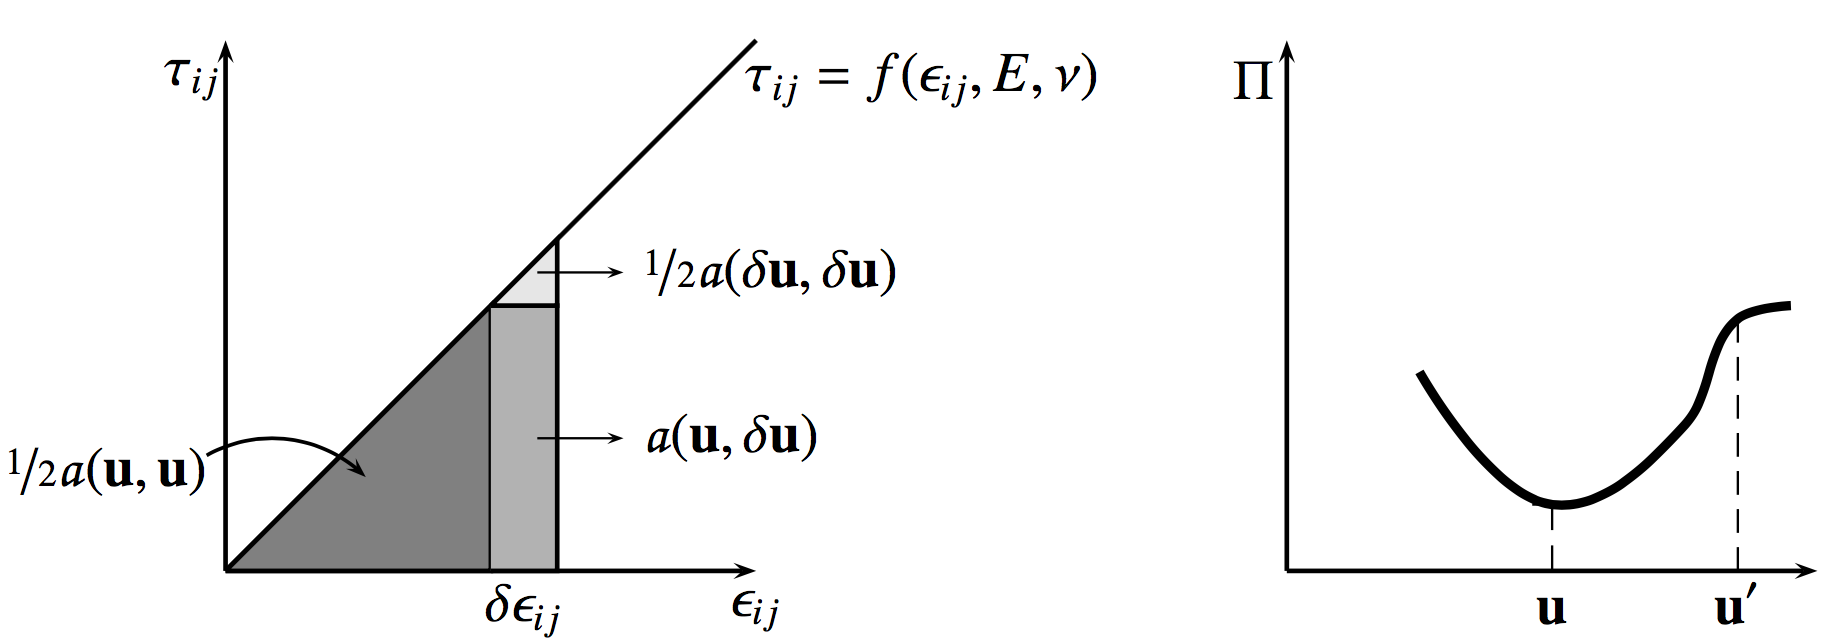
\includegraphics[scale=0.4]{ch4/2}
	\captionof{figure}{}
	\label{fig:4.2}
	\end{center}
	
	This is represented on \autoref{fig:4.2} left where $\delta W(\bm{u}) \approx a(\bm{u}, \delta \bm{u})$ since $a$ is symmetric and $\frac{1}{2}a(\delta \bm{u}, \bm{u})$ is a second order that can be neglected. We have:
	
	\begin{center}
	\theor{
	\textbf{Variational formulation of the virtual displacement theorem}
	
	\begin{equation}
	\delta \Pi = \delta (a(\bm{u},\bm{u}) -\varphi (\bm{u})) = \delta (U+W) = 0 \mbox{ at equilibrium,}
	\end{equation}
	
	where $\Pi$ is the \textbf{total potential energy}. 
	}
	\end{center}
	
	The total potential energy is stationary for variations of admissible displacements. This is a \textbf{minimum} formulation:
	
	\begin{proof}
	Let's define another kinematically admissible displacement $\bm{u'= u+v},$ where $\bm{v}$ is a kinematically homogeneous displacement field. The definition of the total potential energy gives: 
	
	\begin{equation}
	\begin{aligned}
	\Pi (\bm{u'}) &= \Pi (\bm{u+v}) = \frac{1}{2} a(\bm{u+v},\bm{u+v}) - \varphi (\bm{u+v})\\ 
	&= \frac{1}{2} a(\bm{u},\bm{u}) + \frac{1}{2} a(\bm{v}, \bm{v}) + a(\bm{u},\bm{v}) - \varphi (\bm{u}) - \varphi (\bm{v})\\
	\Pi(\bm{u}) &= \frac{1}{2} a(\bm{u},\bm{u}) - \varphi (\bm{u})\\
	\Rightarrow \Pi (\bm{u'}) -\Pi(\bm{u}) &=  \frac{1}{2} a(\bm{v}, \bm{v}) + \cancel{a(\bm{u},\bm{v}) - \varphi (\bm{v})} 
	\end{aligned}
	\end{equation}
	
	where the last two terms vanishes since $\bm{v}$ is kinematically homogeneous. The only remaining term is always $\geq 0$, proving that the total potential energy is a minimum at the solution.
	\end{proof}
	